
\documentclass[a4paper,11pt]{article}
\usepackage{latexsym}
\usepackage{xcolor}
\usepackage{float}
\usepackage{ragged2e}
\usepackage[empty]{fullpage}
\usepackage{wrapfig}
\usepackage{lipsum}
\usepackage{tabularx}
\usepackage{titlesec}
\usepackage{geometry}
\usepackage{marvosym}
\usepackage{verbatim}
\usepackage{enumitem}
\usepackage[hidelinks]{hyperref}
\usepackage{fancyhdr}
\usepackage{fontawesome5}
\usepackage{multicol}
\usepackage{graphicx}
\usepackage{cfr-lm}
\usepackage[T1]{fontenc}
\setlength{\multicolsep}{0pt} 
\pagestyle{fancy}
\fancyhf{} % clear all header and footer fields
\fancyfoot{}
\renewcommand{\headrulewidth}{0pt}
\renewcommand{\footrulewidth}{0pt}
\geometry{left=1.4cm, top=0.8cm, right=1.2cm, bottom=1cm}
% Adjust margins
%\addtolength{\oddsidemargin}{-0.5in}
%\addtolength{\evensidemargin}{-0.5in}
%\addtolength{\textwidth}{1in}
\usepackage[most]{tcolorbox}
\tcbset{
	frame code={}
	center title,
	left=0pt,
	right=0pt,
	top=0pt,
	bottom=0pt,
	colback=gray!20,
	colframe=white,
	width=\dimexpr\textwidth\relax,
	enlarge left by=-2mm,
	boxsep=4pt,
	arc=0pt,outer arc=0pt,
}

\urlstyle{same}

\raggedright
\setlength{\tabcolsep}{0in}

% Sections formatting
\titleformat{\section}{
  \vspace{-4pt}\scshape\raggedright\large
}{}{0em}{}[\color{black}\titlerule \vspace{-7pt}]

%-------------------------
% Custom commands
\newcommand{\resumeItem}[2]{
  \item{
    \textbf{#1}{\hspace{0.5mm}#2 \vspace{-0.5mm}}
  }
}

\newcommand{\resumePOR}[3]{
\vspace{0.5mm}\item
    \begin{tabular*}{0.97\textwidth}[t]{l@{\extracolsep{\fill}}r}
        \textbf{#1}\hspace{0.3mm}#2 & \textit{\small{#3}} 
    \end{tabular*}
    \vspace{-2mm}
}

\newcommand{\resumeSubheading}[4]{
\vspace{0.5mm}\item
    \begin{tabular*}{0.98\textwidth}[t]{l@{\extracolsep{\fill}}r}
        \textbf{#1} & \textit{\footnotesize{#4}} \\
        \textit{\footnotesize{#3}} &  \footnotesize{#2}\\
    \end{tabular*}
    \vspace{-2.4mm}
}

\newcommand{\resumeProject}[4]{
\vspace{0.5mm}\item
    \begin{tabular*}{0.98\textwidth}[t]{l@{\extracolsep{\fill}}r}
        \textbf{#1} & \textit{\footnotesize{#3}} \\
        \footnotesize{\textit{#2}} & \footnotesize{#4}
    \end{tabular*}
    \vspace{-2.4mm}
}

\newcommand{\resumeSubItem}[2]{\resumeItem{#1}{#2}\vspace{-4pt}}

% \renewcommand{\labelitemii}{$\circ$}
\renewcommand{\labelitemi}{$\vcenter{\hbox{\tiny$\bullet$}}$}

\newcommand{\resumeSubHeadingListStart}{\begin{itemize}[leftmargin=*,labelsep=0mm]}
\newcommand{\resumeHeadingSkillStart}{\begin{itemize}[leftmargin=*,itemsep=1.7mm, rightmargin=2ex]}
\newcommand{\resumeItemListStart}{\begin{justify}\begin{itemize}[leftmargin=3ex, rightmargin=2ex, noitemsep,labelsep=1.2mm,itemsep=0mm]\small}

\newcommand{\resumeSubHeadingListEnd}{\end{itemize}\vspace{2mm}}
\newcommand{\resumeHeadingSkillEnd}{\end{itemize}\vspace{-2mm}}
\newcommand{\resumeItemListEnd}{\end{itemize}\end{justify}\vspace{-2mm}}
\newcommand{\cvsection}[1]{%
\vspace{2mm}
\begin{tcolorbox}
    \textbf{\large #1}
\end{tcolorbox}
    \vspace{-4mm}
}

\newcolumntype{L}{>{\raggedright\arraybackslash}X}%
\newcolumntype{R}{>{\raggedleft\arraybackslash}X}%
\newcolumntype{C}{>{\centering\arraybackslash}X}%
%---- End of Packages and Functions ------

%-------------------------------------------
%%%%%%  CV STARTS HERE  %%%%%%%%%%%
%%%%%% DEFINE ELEMENTS HERE %%%%%%%
\newcommand{\name}{Shuvam Banerji Seal} % Your Name
\newcommand{\course}{2nd Year BS-MS Student} % Your Program
\newcommand{\roll}{22MS076} % Your Roll No.
%\newcommand{\phone}{xxxxxxxxxx} % Your Phone Number
\newcommand{\emaila}{sbs22ms076@iiserkol.ac.in} %Email 1
%\newcommand{\emailb}{officialemail@iiitg.ac.in} %Email 2




\begin{document}
\fontfamily{cmr}\selectfont
%----------HEADING-----------------


\parbox{2.35cm}{%
%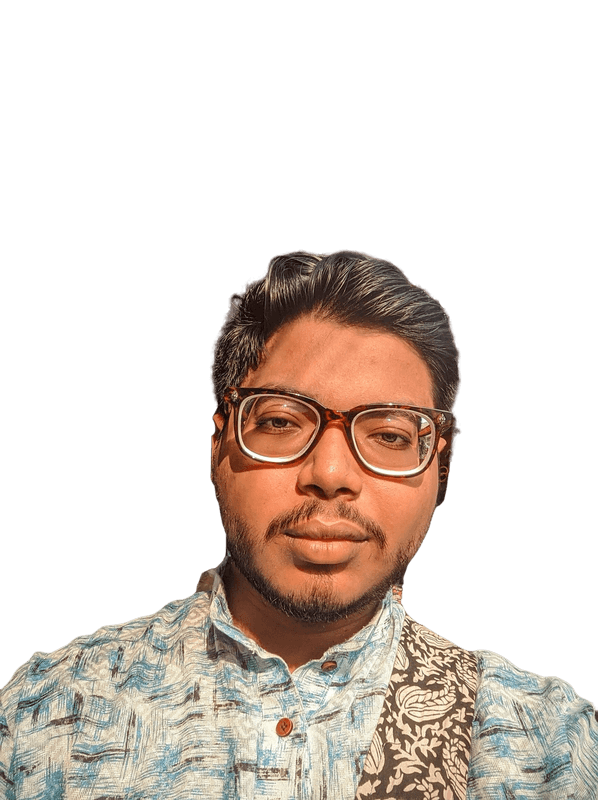
\includegraphics[width=2cm,clip]{dp2.png}
}
\parbox{\dimexpr\linewidth-2.8cm\relax}{
\begin{tabularx}{\linewidth}{L r} \\
  \textbf{\Large \name} & \\
  {Roll No.: \roll} & \href{mailto:\emaila}{\raisebox{0.0\height}{\footnotesize \faEnvelope}\ {\emaila}} \\
  \course &  \href{https://github.com/Shuvam-Banerji-Seal}{\raisebox{0.0\height}{\footnotesize \faGithub}\ {https://github.com/Shuvam-Banerji-Seal}} \\
  {Indian Institute of Science Education and Research - Kolkata} & \href{https://www.linkedin.com/in/mastersbs}{\raisebox{0.0\height}{\footnotesize \faLinkedin}\ {https://www.linkedin.com/in/mastersbs}}
\end{tabularx}
}
% \parbox{3.0cm}{%
% \flushright \includegraphics[width=2cm,clip]{nitp_logo.png}
% }




%-----------EDUCATION-----------
\section{\textbf{Education}}
  \resumeSubHeadingListStart
    \resumeSubheading
      {Indian Institute of Science Education and Research - Kolkata}{CGPA: 8.84}
      {BS-MS with Physics, Chemistry and Mathematics as Pre-Majors}{2022- 2027(Expected)}
    \resumeSubheading
      {Calcutta University}{CGPA: 8.308}
      {B.Sc Honours in Physics (Only 1st Year)}{2021-2022}
    \resumeSubheading
      {Jodhpur Park Boys' High School}{Percentage: 83\%}
      {Physics, Mathematics, Chemistry, Computer Science under WBCHSE}{2019-2021}
      \resumeSubheading
      {The New Horizon High School}{Percentage: 83.75\%}
      {Engligh Medium Schooling under WBBSE}{2009-2019}
  \resumeSubHeadingListEnd
\vspace{-5.5mm}
%



%-----------EXPERIENCE-----------------
\section{\textbf{Experience}}
  \resumeSubHeadingListStart
    \resumeSubheading
      {Educator}{Kolkata}
      {Self-Employed}{2018-Present day}
      
      \resumeItemListStart
    \item \textbf{Subjects Taught :}  Computer Science (+2 Level), English (+2 Level), Physics (+2 Level), Chemistry(+2 Level), Economics(+2 Level), Social Sciences(Secondary Level
    \item \textbf{Special Courses Taught:} An Extensive Analysis of Figures of Speech, Outdoor Instant Poetry Composition, A full Course on HTML, Linear Data Structures for +2 Students, and a few more.
    \item \textbf{Skills Acquired:} Good Communication Skills, Child Psychology Analysis, Hand-writing Analysis, Good Presentation Skills.
    \resumeItemListEnd
    
    \vspace{-3.0mm}
    
    \resumeSubheading
      {PC Builder and Repairer}{Kolkata}
      {Self-Employed}{2021- Present Day}
      \resumeItemListStart
    \item \textbf{Soft Skills: }{From casual to office and even gaming PC(s), with good Asthetic design and smart cable management, along with polite Customer Service}
    \item \textbf{Practical Skills: } Understanding of Computer Hardware and Software skills like BIOS/UEFI calibration i.e. Voltage and current parameters, OS installation, and so on.
    \resumeItemListEnd

    \resumeSubheading
      {Creative Writer}{Kolkata}
      {Poet}{2020}
      \vspace{-2.0mm}
      \resumeItemListStart
    \item \textbf{Title: }MindScapes | \textbf{ISBN-10 } 9389923204 | \textbf{ISBN-13} 978-9389923209
    \resumeItemListEnd
    
    \resumeSubheading
      {Anicon 2.0 (IISER-K)}{Kalyani}
      {Event Organizer}{2023}
      \vspace{-2.0mm}
      \resumeItemListStart
    \item \textbf{Responsibilities: } Event Planning, Volunteer Co-ordination, Event Hosting
    \resumeItemListEnd
    
    \resumeSubheading
      {Social Welfare}{Kolkata and Kalyani}
      {}{2021-2023}
      \vspace{-2.0mm}
      \resumeItemListStart
    \item Food Resource Distributor during Covid Pandemic
    \item Providing free education for financially challenged students under Ek-Pehal (IISER-Kolkata)
    \resumeItemListEnd



%-----------PROJECTS-----------------
\section{\textbf{Research Projects}}
\resumeSubHeadingListStart

    \resumeProject
      {Simulation of Symmetries with the Changes in the Fine Structures} %Project Name
      {The aim is to draw out abstract symmetries when the fundamental constants change itself.} %Project Name, Location Name
      {2023 (ongoing)} %Event Dates

%      \resumeItemListStart
 %       \item {Python }
  %      \item {More description on the project(The output you achieved by working on the project)}
   % \resumeItemListEnd
    %\vspace{-2mm}
    
        
      
  \resumeSubHeadingListEnd
\vspace{-5.5mm}



%-----------Technical skills-----------------
\section{\textbf{Technical Skills and Interests}}
 \begin{itemize}[leftmargin=0.05in, label={}]
    \small{\item{
     \textbf{Programming Languages}{: Python | C/C++ | Java | Javascript | Rust | QBASIC | GWBASIC } \\
     \textbf{Developer and Research Tools}{: HTML | CSS | PHP(Basics) | LaTeX | Scilab | Origin Pro | GNUPlot | VMD | LAMMPS } \\
     %\textbf{Frameworks}{: } \\
     \textbf{Cloud/Databases}{: MongoDB | MySQL } \\
     \textbf{Soft Skills}{: Fluent in Communication | Public Speaker | Team Co-ordinator | Understanding team Psyche and Motivation to direct the flow } \\
     \textbf{Coursework}{: Online Certificate Course in Python Programming from National Institute of Electronics and Information Technology | CS50 from Harvard (Informal) | Data Structures and Implementation (NPTEL) | QIQT 2023  \\
     \textbf{Areas of Interest}{: Algorithm Development | Quantum Physics and Computation | Molecular Dynamics} \\
     \textbf{Miscellaneous:} {HTML E-mailing | Front-end Designing | Figma | Canva | Spreadsheets | XML scripting | Bash }
    }}
 \end{itemize}
 \vspace{-16pt}



%-----------Positions of Responsibility-----------------



%-----------Achievements-----------------
\section{\textbf{Achievements}}
\vspace{-0.4mm}
\resumeSubHeadingListStart
\resumePOR{Qualified JEE Mains and Advanced} % Award
    {   Ranked in Top 0.1 fraction of Candidates} % Event
    {2022} %Event Year
\resumePOR{Qualified IAT}{Ranked in top 2000 candidates}{2022}

\resumePOR{Qualified WBJEE} % Award
    {   Ranked in Top 0.05 fraction of Candidates} % Event
    {2022} %Event Year

\resumePOR{Olympiads} % Award
    { SOF IEO International Rank : 536, Zonal Rank : 29} % Event
    {2019-20} %Event Year
\resumePOR{Olympiads} % Award
    { SOF IEO International Rank : 331, Regional Rank : 157} % Event
    {2020-21}
\resumePOR{Olympiads} % Award
    { SOF NSQ International Rank : 346, Zonal Rank : 22} % Event
    {2020-21}
\resumePOR{Zonal Topper} % Award
    {Mimansa by IISER Pune : Contributed in Mathematics} % Event
    {2024}
\resumeSubHeadingListEnd

\resumeSubHeadingListEnd

\vspace{-5mm}
\setlength{\footskip}{4.08003pt}
 

%-------------------------------------------

%-----------Achievements-----------------
\section{\textbf{Honours And Rewards}}
\vspace{-0.4mm}
\resumeSubHeadingListStart
\resumePOR{Reliance Foundation Undergraduate Scholar} % Award
    {} % Event
    {2023} %Event Year
   % \resumeSubHeadingListEnd

\resumePOR{Most Creative Use of MatLab} % Award
    { StatusCode0 Hackathon organised by IIIT Kalyani} % Event
    {2023} %Event Year
\resumePOR{Best Speaker (NanoTechnology)} % Award
    {World Science Conference} % Event
    {2020} %Event Year
\resumeSubHeadingListEnd

\resumeSubHeadingListEnd

\vspace{-5mm}
\setlength{\footskip}{4.08003pt}
 

%-------------------------------------------
\section{\textbf{Extra-Curricular}}
\vspace{-0.4mm}
\resumeSubHeadingListStart
\resumePOR{District Level Debator} % Award
    {Runner-Up, debate organized by West Bengal Mathematical Society} % Event
    {2018} %Event Year
   % \resumeSubHeadingListEnd
\resumePOR{Art and Painting} % Award
    { 4th Year with major works in Stroke Art and Portraits} % Event
    {2016-2020} %Event Year
\resumePOR{Karate} % Award
    { Shotokan Style Under Debkingkor Ghosh Sensei} % Event
    {2014-18}
\resumePOR{Debates and Extempores} % Award
    { Participated in various such events} % Event
    {2014-Present Day}
\resumePOR{Quiz} % Award
    { Participated in various Quizzes all through-out school life} % Event
    {2014-21}
\vspace{-5mm}
\setlength{\footskip}{4.08003pt}


\resumeSubHeadingListEnd

\end{document}
